% Two optional motivation frames with real-world examples.

\begin{frame}{Real-World Example 1: Image Color Quantization}
  \small
  \begin{columns}[c,onlytextwidth]
    \column{.69\textwidth}
      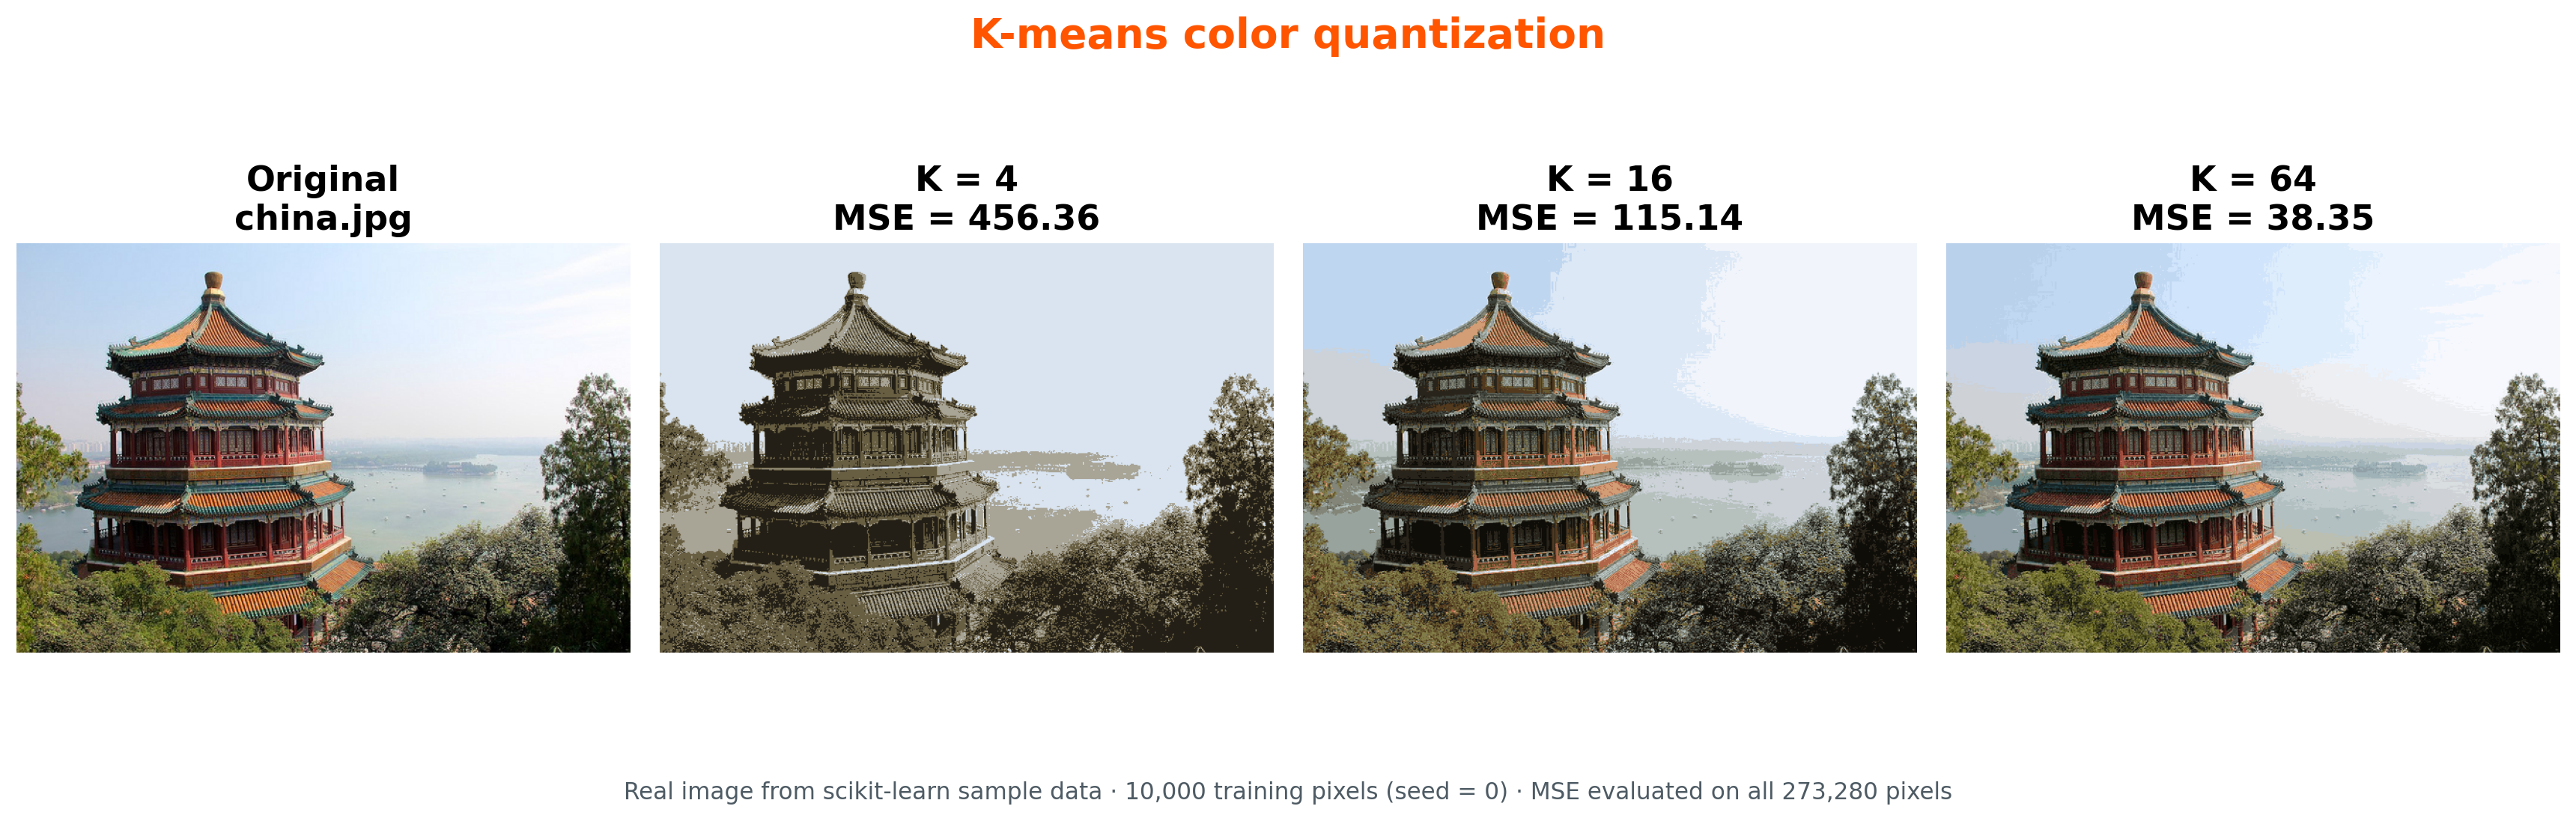
\includegraphics[width=.98\textwidth]{assets/motivation/kmeans_color_quantization.png}
    \column{.27\textwidth}
      \textbf{One observation}
      \[
        x_i=(R_i,G_i,B_i)
      \]
      one pixel in RGB space.

      \vspace{.06cm}
      \textbf{Clusters}

      pixels assigned to the same palette color.

      \vspace{.06cm}
      \textbf{Purpose}

      compact storage, transmission, and display.
  \end{columns}

  \src{Source: \href{https://scikit-learn.org/stable/auto_examples/cluster/plot_color_quantization.html}{scikit-learn color quantization example}.}
\end{frame}

\begin{frame}{Real-World Example 2: Customer Segmentation}
  \small
  \begin{columns}[c,onlytextwidth]
    \column{.46\textwidth}
      \IfFileExists{assets/motivation/shoppers.jpg}{%
        \includegraphics[width=.98\textwidth]{assets/motivation/shoppers.jpg}%
      }{%
        \fbox{\parbox[c][4.3cm][c]{.92\linewidth}{\centering Insert a customer or shopping image here}}%
      }

    \column{.48\textwidth}
      \textbf{One observation}

      a standardized feature vector for one customer, such as recency, purchase frequency, spend, and product mix.

      \vspace{.14cm}
      \textbf{Clusters}

      customers with similar observed behavior.

      \vspace{.14cm}
      \textbf{After clustering}

      compare retention, offers, or service policies across segments.
  \end{columns}

  \src{Photo source: Wikimedia Commons; public-domain NIH image.}
\end{frame}
